%%%%%%%%%%%%%%%%%%%%%%%%%%%%%%%%%%%%%%%%%%%%%%%%%%%%%%%%%%%%%%%%%%%%%%%%%%%%%
\section{Introduction}
\label{sec:introduction}
%%%%%%%%%%%%%%%%%%%%%%%%%%%%%%%%%%%%%%%%%%%%%%%%%%%%%%%%%%%%%%%%%%%%%%%%%%%%%

%Emerging technologies such as SDN and NFV are great promises. If succeeding at large-scale, they should change the development and operation of computer networks. But, enabling technologies such as virtualization still pose challenges on performance,  reliability, and security\cite{nfv-challenges}. Since virtualization brings some degradation on latency and throughput it must be kept as small as possible.  On stability and resilience, dedicated hardware has a more foreseeable behaviour than VNFs. Along with this, newer extra layers (hypervisor, orchestrator) may generate newer security weaknesses.  Thus, guarantee  the Service Layer Agreements on emerging scenarios is now a harder question. Applications may have a huge performance degradation processing small packets\cite{comparative-trafficgen-tools}\cite{performance-trafficgen}. As conclude by many investigations, realistic and burstiness traffic impacts on bandwidth measurement accuracy\cite{background-traffic-matter}\cite{legotg-paper}. Also, realistic workload generators are essential security research. It can provide training and validation of many tasks, such as  anomaly and thread detection, intrusion and malicious workload.  Moreover, all these aspects have to be validated at actual traffic rates. Thus, there is a demand for tests able to address realism at high throughput rates.


Emerging technologies such as SDN and NFV are great promises. If succeeding at large-scale, they should change the development and operation of computer networks. But, enabling technologies such as virtualization still pose challenges on performance,  reliability, and security\cite{nfv-challenges}.  Thus, guarantee  the Service Layer Agreements on emerging scenarios is now a harder question. Applications may have a huge performance degradation processing small packets\cite{comparative-trafficgen-tools}. As conclude by many investigations, realistic and burstiness traffic impacts on bandwidth measurement accuracy\cite{legotg-paper}. Also, realistic workload generators are essential security research\cite{ditg-paper}. Thus, there is a demand for tests able to address realism at high throughput rates.  

The open-source community offers a huge variety of workload generators and benchmarking tools \cite{ditg-paper}\cite{validate-trafficgen}. Each tool uses different methods on traffic generation, focusing on a certain aspects. Some traffic generator tools provide support emulation of single  application workloads. But this is not enough to describe an actual Service Provider(ISP) load or even a LAN scenario. Other tools work as packet replay engines, such as TCPreplay and TCPivo. Although in that way is possible to produce a realistic workload at high rates, it comes with some issues. First, the storage space required becomes huge for long-term and high-speed traffic capture traces. Also, obtaining good traffic traces sometimes is hard, due privacy issues and fewer good sources. Many tools aim the support of a larger set of protocols and high-performance such Seagull and Ostinato. Many are also able to control inter-departure time and packet size using stochastic models, like D-ITG\cite{ditg-paper} and MoonGen. They can provide a good control of the traffic, and high rates. But, in this case, selecting a good configuration is by itself a research project, since how to use each parameter to simulate a specific scenario is a hard question \cite{selfsimilar-ethernet}. It is a manual process and demands implementation of scripts or programs leveraging human (and scarce) expertise on network traffic patterns and  experimental evaluation. Some tools like Swing and Harpoon, try to use the best of both worlds. Both use capture traces to set intern parameters, enabling an easier configuration. Also, Swing uses complex multi-levels which are able to provide a high degree of realism\cite{swing-paper}. But they have their issues as well. Harpoon does not configure parameters at packet level\cite{harpoon-paper} and is not supported by newer Linux kernels. Swing\cite{swing-paper} aims to generate realistic background traffic, not offering high throughput \cite{swing-paper} \cite{legotg-paper}. As is possible to see, this a result of the fact that its traffic generation engine is coupled to its modeling framework. You can't opt to use a newer/faster packet generator. The only way of replacing the traffic engine is changing and recompiling the original code. And this is a hard task.

This project aims to create a framework able solve many of presented issues.  It must be able to "learning" patterns and characteristics of real network traffic traces. Then, using packet generators and accelerators it should reproduce a network traffic with similar  characteristics. Based on observation of live captures or PCAP files, the software must choose the bests parametrized stochastic functions (from a list) to fit the data. These parametrized stochastic functions along with collected header features (such as protocols and addresses) will be record in a machine-readable file (such as XML or JSON) we baptise as a Compact Trace Descriptor (CTD). This data must serve as input for an API of a traffic generator. So it will be possible to control packet parameters, and flow's behaviours, through different APIs. Also, and speed-up may be achieved, though the use of DPDk's KNI interfaces\footnote{ \url{http://dpdk.org/doc/guides/sample_app_ug/kernel_nic_interface.html} }. So, the main goal is to offer an easier configuration, realism, at a higher speed than the available platforms today. Also, it will add programmability and abstraction to the traffic generation, since the user may edit or create a custom traffic descriptor in a platform agnostic way. The the intermediate layer of the figure ~\ref{fig:arquitetura-layer} summarize, goal of the project in an illustrative way.

\begin{figure}[H]
        {\centering
        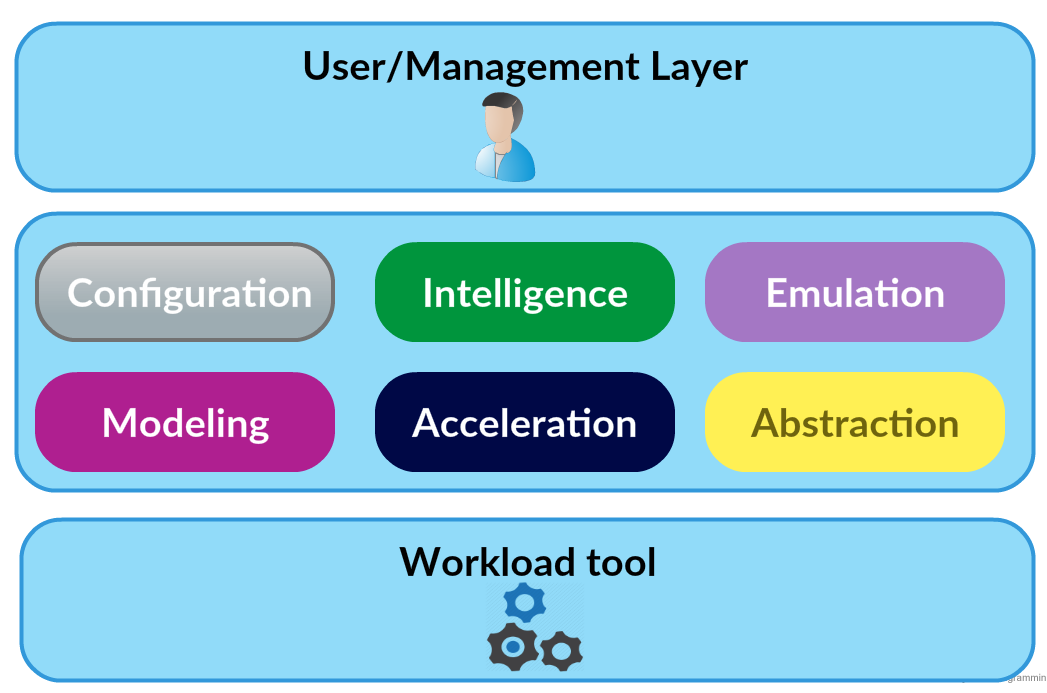
\includegraphics[height=35mm]{figures/arquitetura-layer.png}
        \caption{Proposal representation in a layer diagram. It automates features such as configuration, modelling, and parametrization, intelligence, emulation, and abstraction through an additional layer.}
        \label{fig:arquitetura-layer}\par}
\end{figure}

%%%%%%%%%%%%%%%%%%%%%%%%%%%%%%%%%%%%%%%%%%%%%%%%%%%%%%%%%%%%%%%%%%%%%%%%%%%%%
\section{Literature review and related work}
\label{sec:literature-review}

%\subsection{Classes of traffic generators}
%\label{subsec:classes-traffic-generators}

A common taxonomy used on traffic generator tools based on the layer of operation. It divides them into four categories\cite{do-you-trust}:

\textit{Application-level/Special-scenarios traffic generators}: they emulate applications behaviours, through stochastic and responsive models. Eg.: Surge, GenSym.

\textit{Flow-level traffic generators}: they emulate features of the flow level, such as file transference and bursts. But do not model applications or packet behaviour.Eg.: Harpoon.

\textit{Packet-level traffic generators}: they model inter-departure time and packet size  through stochastic distributions. They focus on performance testing. Eg: D-ITG\cite{ditg-paper}, Ostinato, Seagull, TG.

\textit{Multi-level traffic generators}: These traffic generators models each mentioned layer, describing user and network behaviour. They generate an accurate background traffic, but usually, have bottlenecks on bandwidth. Eg.: Swing\cite{swing-paper}.

%Another important key point is that not every stochastic is able  to represent Ethernet traffic. As showed in many researchers, the Ethernet is self-similar and has a high variability. Self-similarity means it has a fractal-like shape. Characteristics seen in a small-scale of time, are expected to be seen on a long scale of time, as well. Other models, such as like Markov and Poisson-batch cannot capture "burstiness" in a long-term time scale. They do not capture, for example, traffic "spikes" on long-range "ripples". This is referred as Long-range dependence or degree of long-range dependence (LRD). One way to identify if a process is self-similar is checking its Hurst parameter, or Hurt exponent H, as a measure of the "burstiness" and LRD. A random process is self-similar and LRD if 0.5 < H < 1. High variability means, in mathematical terms, an infinite variance. Processes with such characteristic are heavy-tailed [19]. In practical terms, that means a sudden discontinuous change can always occur.  Heavy tail means that a stochastic distribution is not exponentially bounded [19]. This means that a value far from the mean does not have a negligible probability of occurrence. Some examples of heavy-tailed probabilistic functions are Weibull, Cauchy, log-normal, and t-distributions. Thus, self-similarity and high variability must be considered in the modelling. 

%\subsection{Related Work}
%\label{subsec:related-work}

Varet et al. \cite{sourcesOnOff-paper} creates an application in C, called SourcesOnOff. It models the activity interval of packet trains using probabilistic distributions. To choose the best stochastic models, the authors captured many traffic traces using TCPdump. Then, they figure out what distribution (Weibull, Pareto, Exponential, Gaussian, etc.) fits better the original traffic traces, using the Bayesian Information Criterion. For this task, they choose the function with the smaller BIC. The smaller this value is, the better the function fits the data. 

Bartlett et al. \cite{legotg-paper} implements a modular framework for composing custom traffic generation. Its goal is making easy the combine of different traffic generators and modulators in different test-beds. It automatizes the process of installation, execution, resource allocation and synchronization using a centralized orchestrator and a software repository. It already has support to many tools, and to add support to new tools is necessary to add and edit two files, called TGblock, and ExFile.

%\begin{figure}[H]
%        {\centering
%        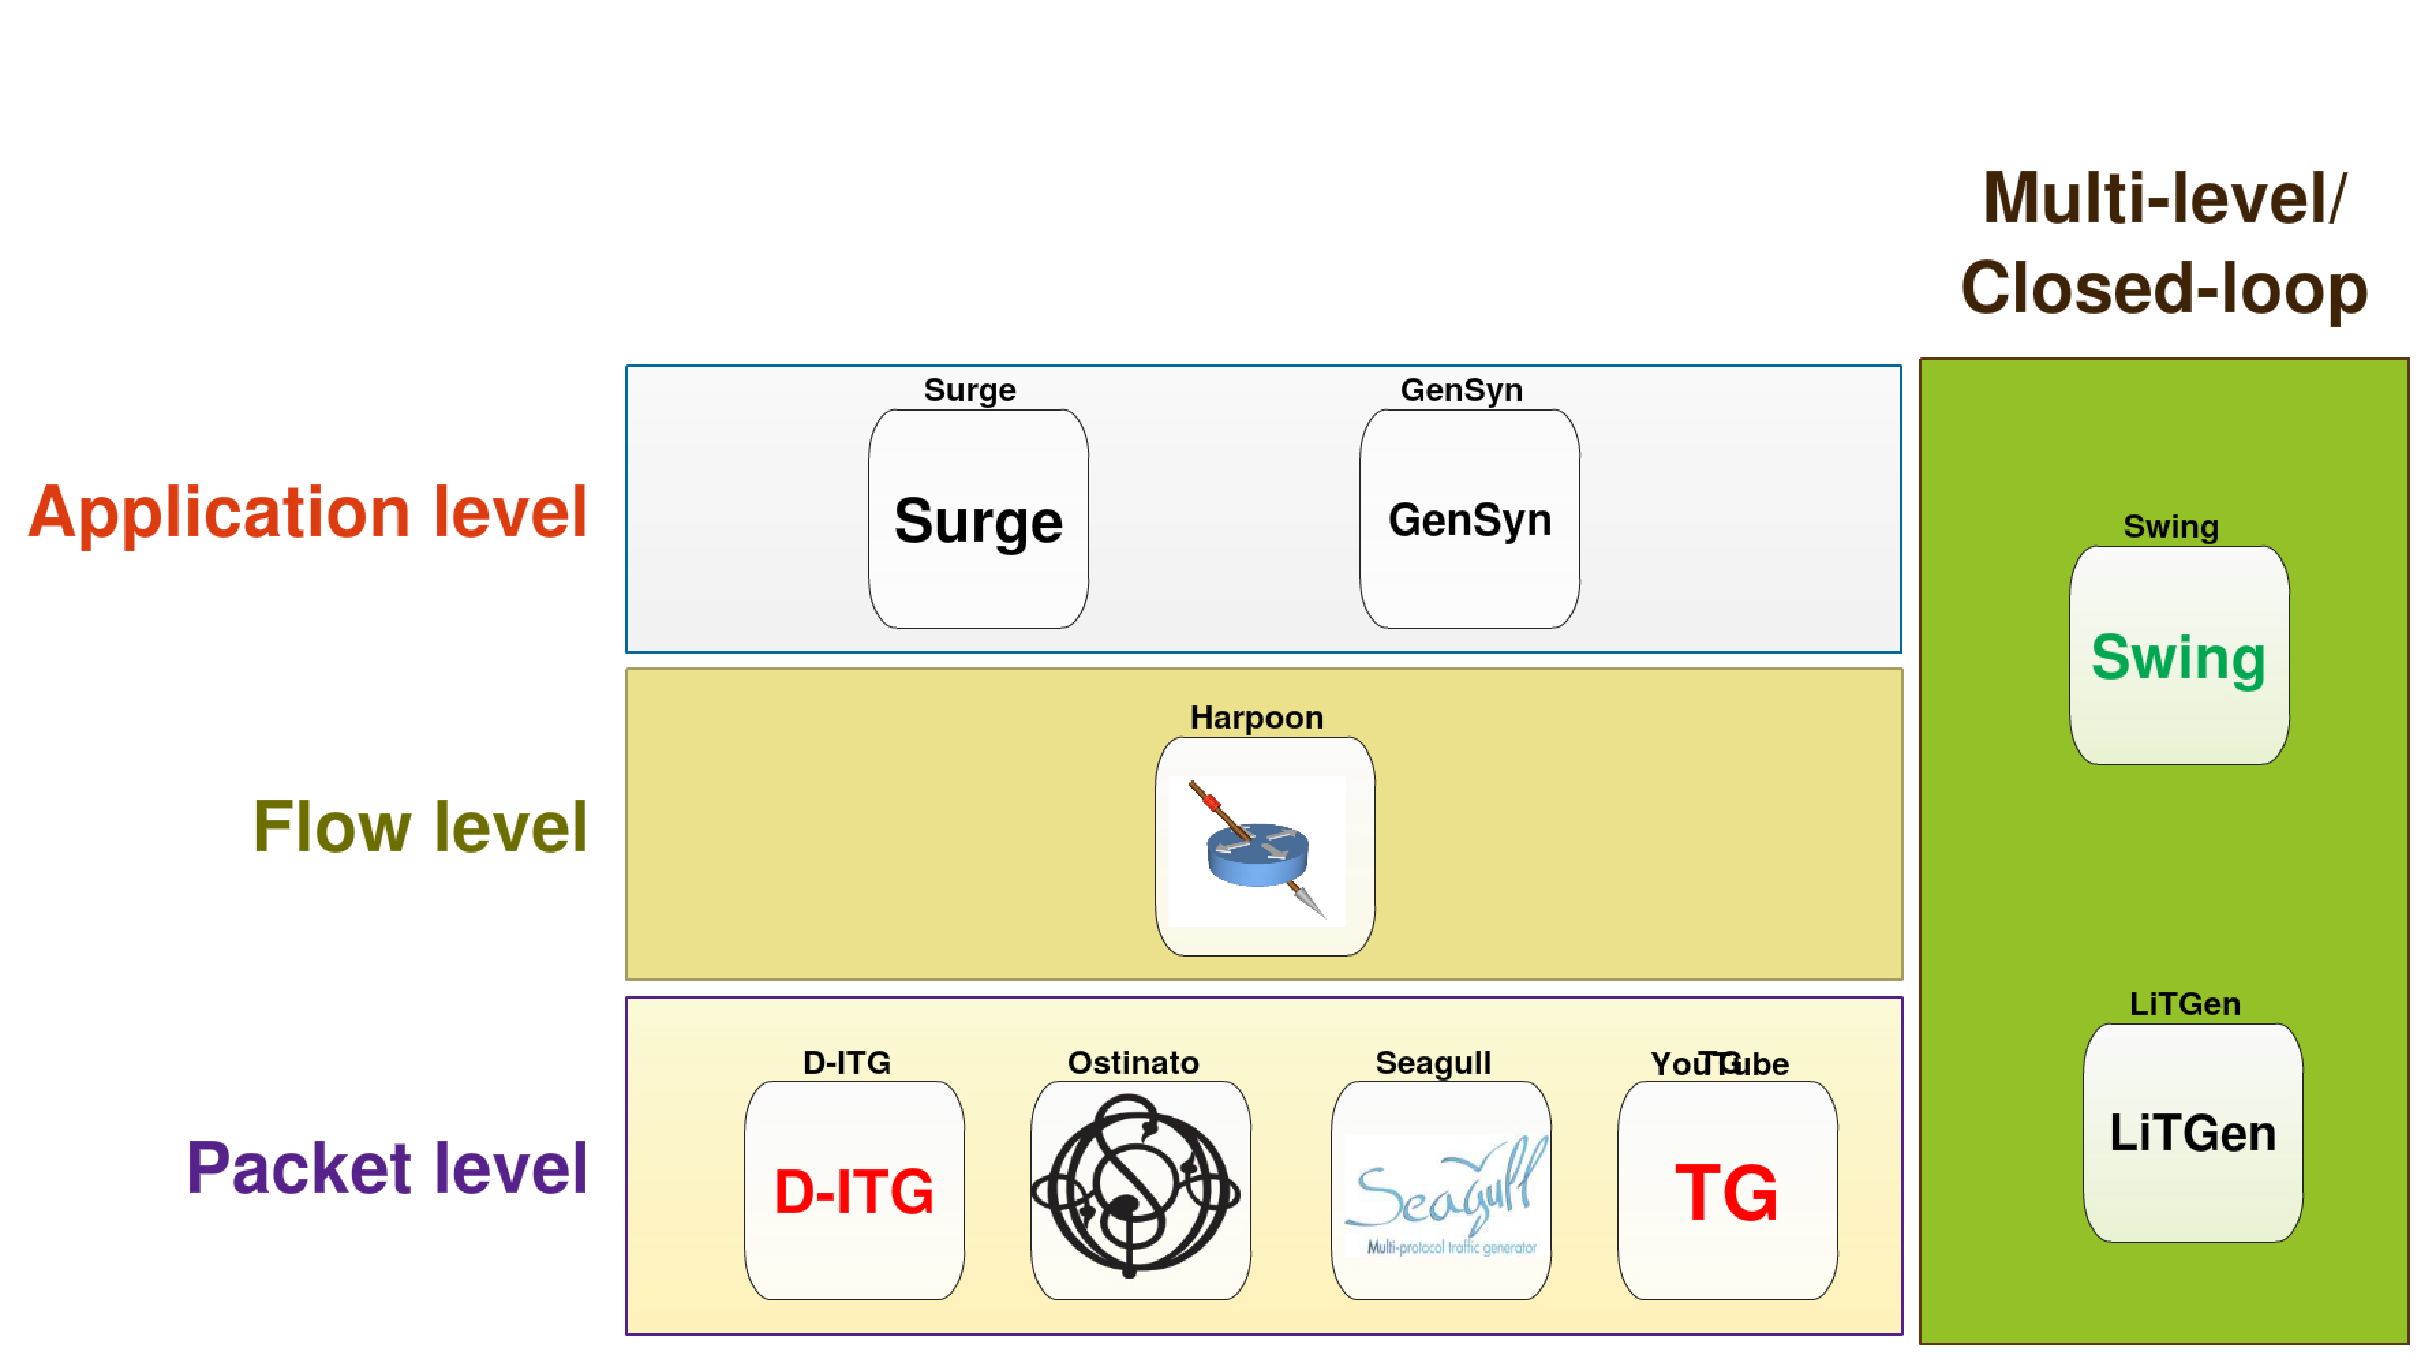
\includegraphics[height=45mm]{figures/types-workload-tools}
%        \caption{}
%        \label{fig:wwwwwwww}\par}
%\end{figure}

%%%%%%%%%%%%%%%%%%%%%%%%%%%%%%%%%%%%%%%%%%%%%%%%%%%%%%%%%%%%%%%%%%%%%%%%%%%%%
\section{System Architecture}
\label{sec:system-architecture-and-requirements}

We developed and architecture that solves the listed issues. It has five components: a Sniffer, an SQLite database, a Trace Analyzer, a Flow Generator, and a Network Traffic Generator as a subsystem.


The Sniffer is responsible collecting data from the network traffic. It extracts data from the packets and stores them in the database. This information can be protocols, packet size, inter-arrival time, flows, and so on. Also, after finishing a capture, this component is the responsible for providing data visualization. It may  work over a PCAP file, or over an Ethernet interface. The prototype version of this component uses tsahrk to capture packets and Shell/Octave scripts. To improve performance and avoid bottlenecks, next implementation will use libtins librarie for packet processing. The criteria to classify the traffic into flows is the same of SDN switches: internet protocol, source/destination addresses, transport protocol, and source/destination transport ports. The framework uses an SQLite database.

The Trace Analyzer is the core of the project. It is the tool responsible for characterizing the trace. Using the stored information, breaks the trace into flows, and parametrize each of them.  The parameters are  header fields and stochastic functions/coefficients for each flow. The component models the behaviour of the trace on flow level and packet level. At the packet level, is possible to model the packet-size and the inter-departure time, during packet bursts (ON times). At the flow level, is possible to control bursts periods, session length,  and the number of bytes delivered. We will use likelihood criterions to choose the best probabilistic function and parameters. Options are the smaller error, Akaike information criterion, and Bayesian information criterion\cite{sourcesOnOff-paper}. It will sort the parametrized functions in a priority list. After the parametrization, the Trace Analyzer records these features in a machine-readable file (XML, JSON) called "Compact trace descriptor".  %This file describes each original traces' flow.

\begin{figure}[H]
        {\centering
        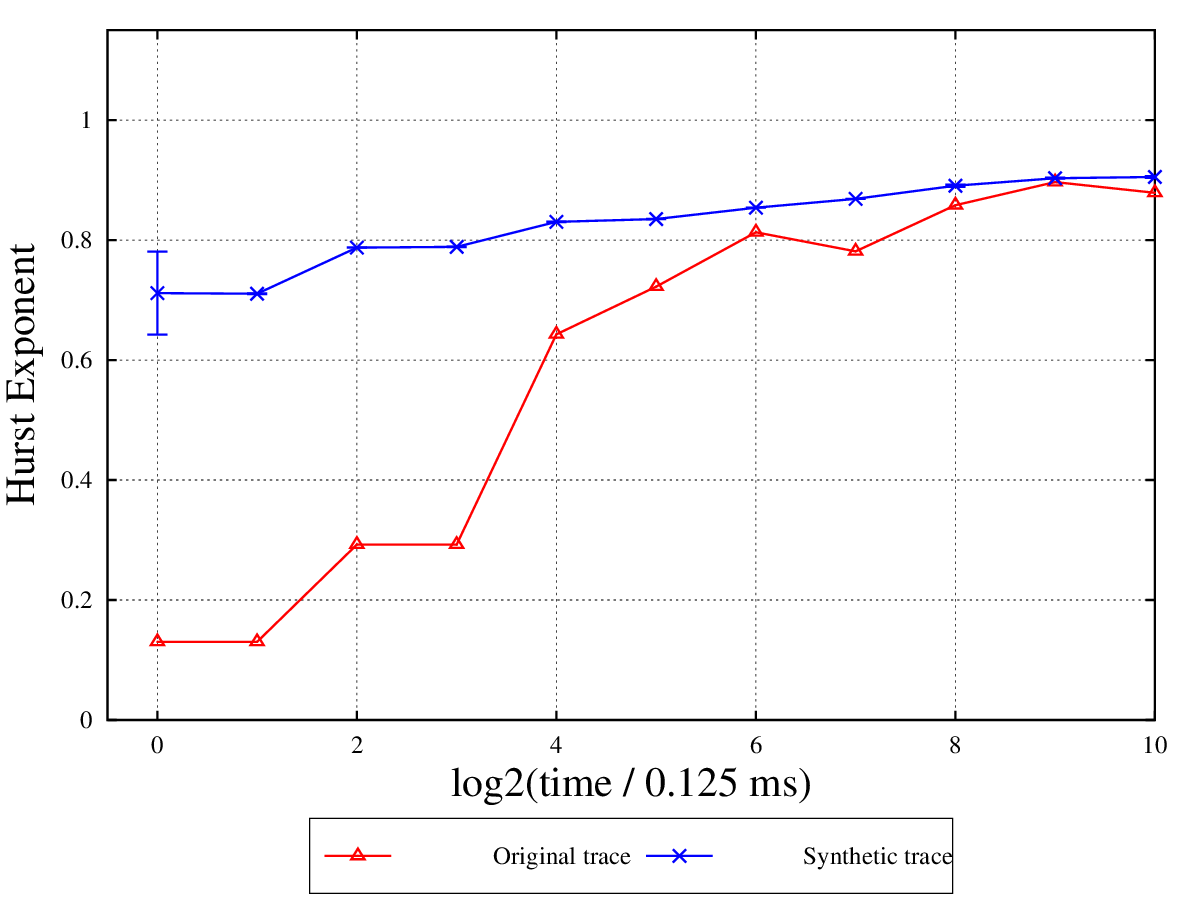
\includegraphics[height=50mm]{figures/qualification-HustExponent.png}
        \caption{Hurst exponent value of original and synthetic traces}
        \label{fig:hurst-exponent}\par}
\end{figure}

The Flow Generator pick these abstract parameters and feed an Ethernet workload generator tool. It crafts each flow in an independent way, in a different thread. The presented prototype just uses the D-ITG API as workload tool.  But it can use any packet-level traffic generator with API or CLI. This component handles the flow level models and parametrizes the packet-level tool underneath. Since each packet-level tool supports a different set of stochastic functions, the Flow Generator should pick the first compatible model from the priority list. But prototype presented here still uses simple models on packet and flow crafting, supporting just constant distributions. But the next release should support at packet-level heavy-tailed\cite{sourcesOnOff-paper} and Poison functions for the inter-departure times, and  bimodal distributions\cite{packet-distribution-model}\cite{udp-flows-model} for the packet size. At the flow level, two different alternatives can be used. Model file transference and session,  such as in Harpoon\cite{harpoon-paper}; or use an envelope process, as suggested by Melo et al\cite{envelope-process-equivalent-bandwidth}.


%\begin{figure}[ht!]
%        {\centering
%        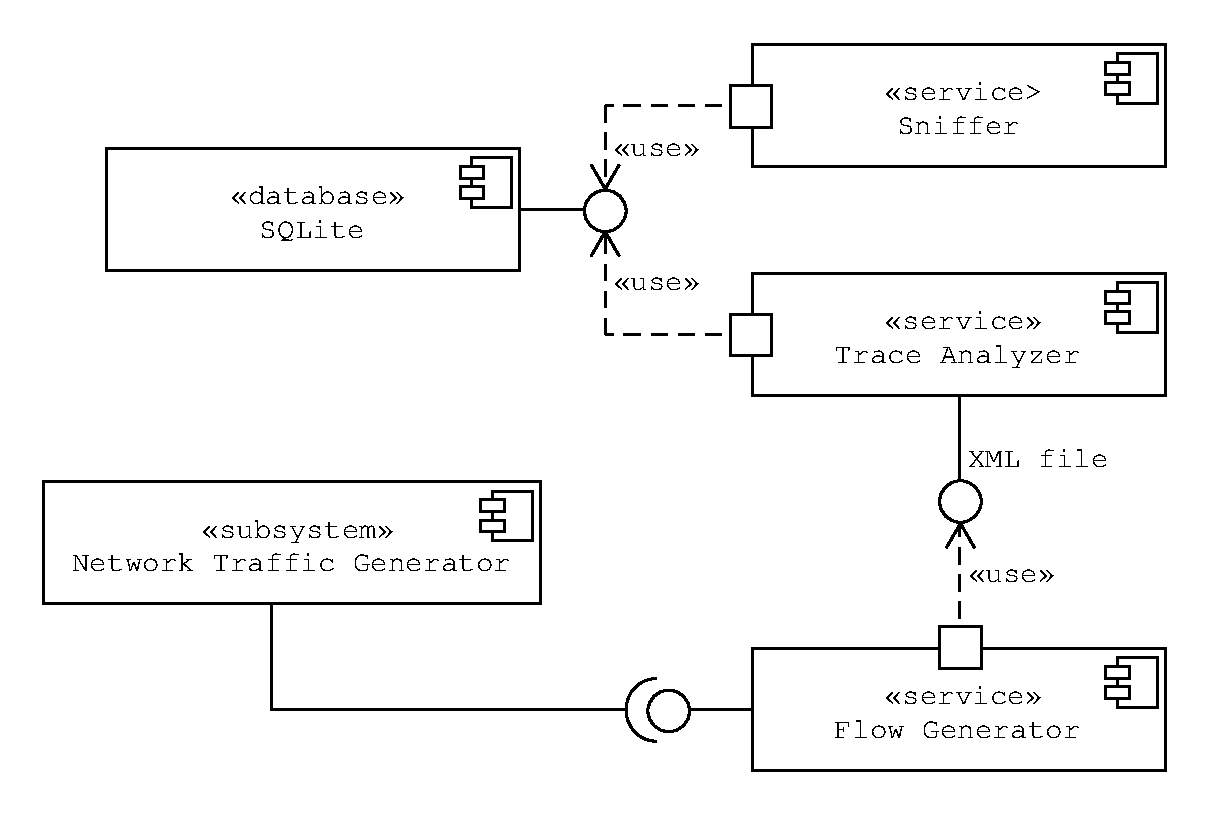
\includegraphics[height=45mm]{figures/Component_Diagram_Alternative.pdf}
%        \caption{}
%        \label{fig:arquitetura-layer}\par}
%\end{figure}

%%%%%%%%%%%%%%%%%%%%%%%%%%%%%%%%%%%%%%%%%%%%%%%%%%%%%%%%%%%%%%%%%%%%%%%%%%%%%
\section{Partial results}
\label{sec:partial-results}

To as proof of concept, we propose a set of tests. We choose them, based on tests used to ensure realism, on related many works \cite{sourcesOnOff-paper} \cite{swing-paper} \cite{legotg-paper}. They aim to ensure realism and similarity. Realism tests measure if a synthetic traffic has expected features of an Ethernet capture. Similarity tests measures if the generated traffic represents specific characteristics of the original one. Here, due the limited space, we will present just two results. The first, which test realism, is the Hurst exponent evaluation. It is able to test the self-similarity of the generated traffic. To be self-similar, a process must have a Hurst exponent between 0.5 and 1 \cite{selfsimilar-ethernet}. Also, usual values of Ethernet traffic lay between 0.8 and 0.9 \cite{selfsimilar-ethernet}.  




Thus a realistic Ethernet traffic must have a Hurst exponent close to the last interval. The second test is Wavelet Multiresolution Energy Analysis. It is able to capture characteristics of the traffic at different time-scales. For example, it enables  visualization of a periodic tendency(decrease) or a self-similar tendency(increase) at a certain time scale. Also, at each point, it represents the mean energy of that signal at that time scale. So, similar Ethernet traffics must have slopes at close time-scales. Also, they must have close energy scales. More close are the curves, more similar are the traces.

The evaluated prototype support just constant functions. It selects the inter-departure time equal to the mean. The packet size is set as the most frequent value. The flow's start time and duration are the same from the observed traffic. We capture the original traffic trace on the laboratory LAN. The results are at figures ~\ref{fig:hurst-exponent} and ~\ref{fig:wavelet-mrea}. On both analysis, the generation of the synthetic trace was repeated 30 times. The keys which serves as input to D-ITG were randomly selected. At  is possible to see that the on both cases the Hurst exponent converge to the same value, close to 0.9. But, on the wavelet multiresolution analysis, both curves still different behaviours.   

% validation figure sample
%\begin{figure}[H]
%    \centering
%    \subfigure[Original]{\label{fig:a}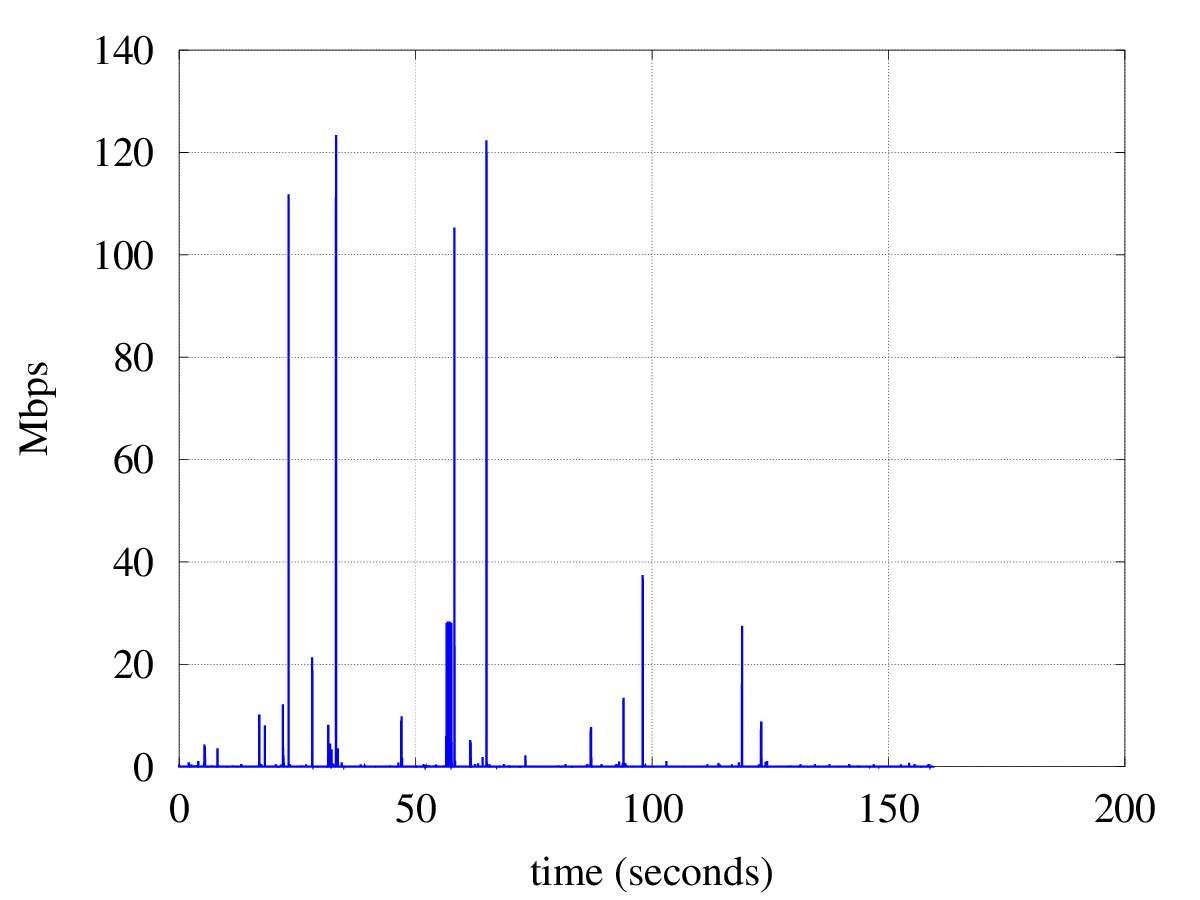
\includegraphics[height=45mm]{figures/Mbps-base}}
%	\subfigure[Synthetic]{\label{fig:b}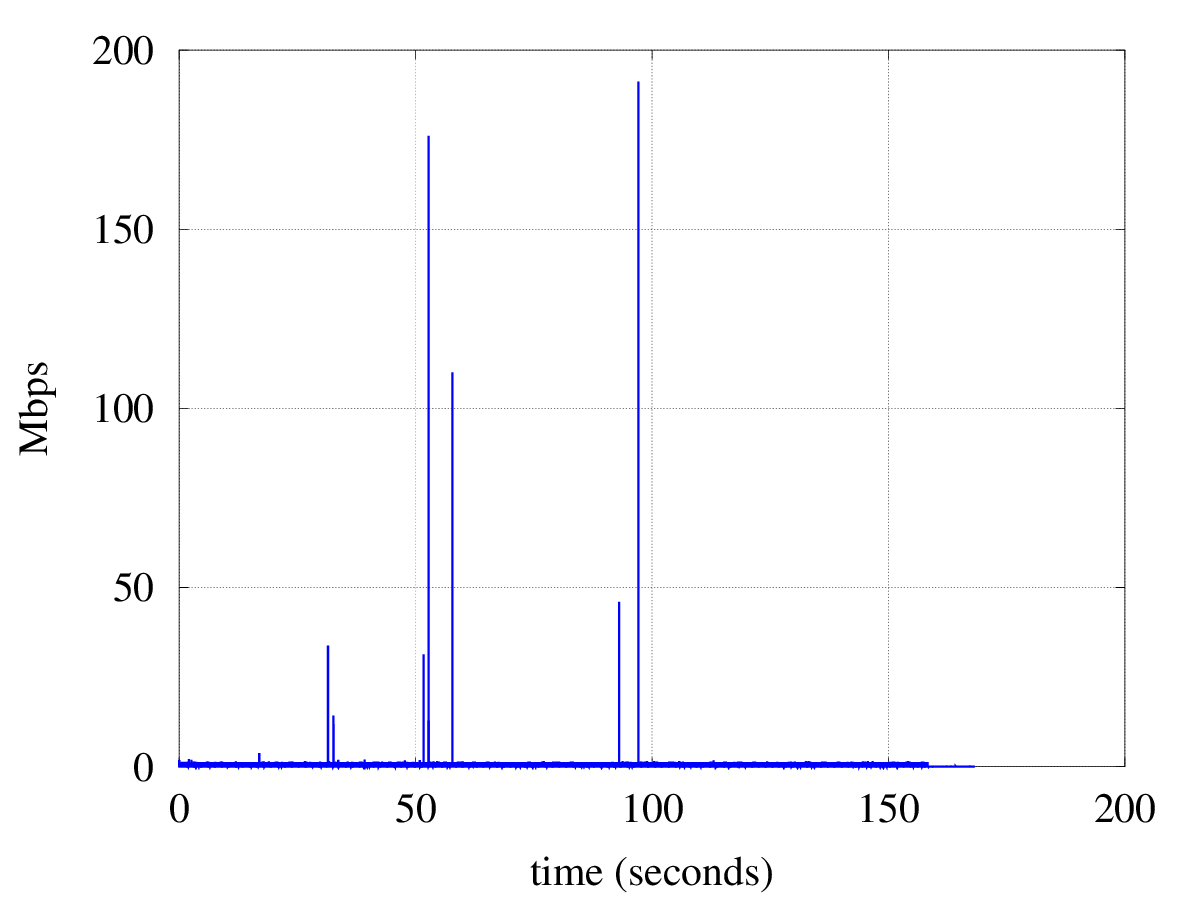
\includegraphics[height=45mm]{figures/Mbps-qualification}}
%    \caption{Bandwidth comparison between original and synthetic traces. Granularity of the plot: 10ms }
%    \label{fig:mbps-comparison}
%\end{figure}

%\begin{figure}[H]
%    \centering
%    \subfigure[Original]{\label{fig:a}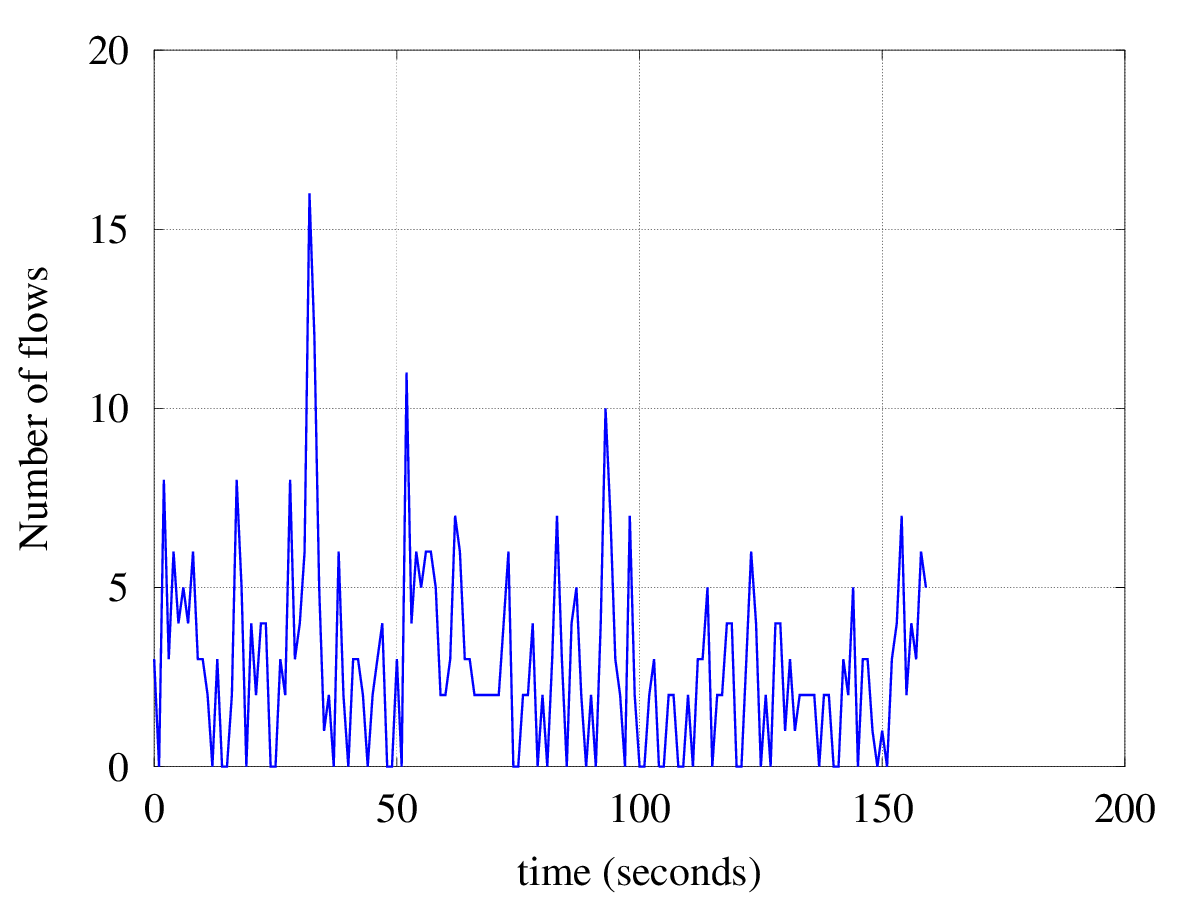
\includegraphics[height=55mm]{figures/Flow-base}}
%	\subfigure[Synthetic]{\label{fig:b}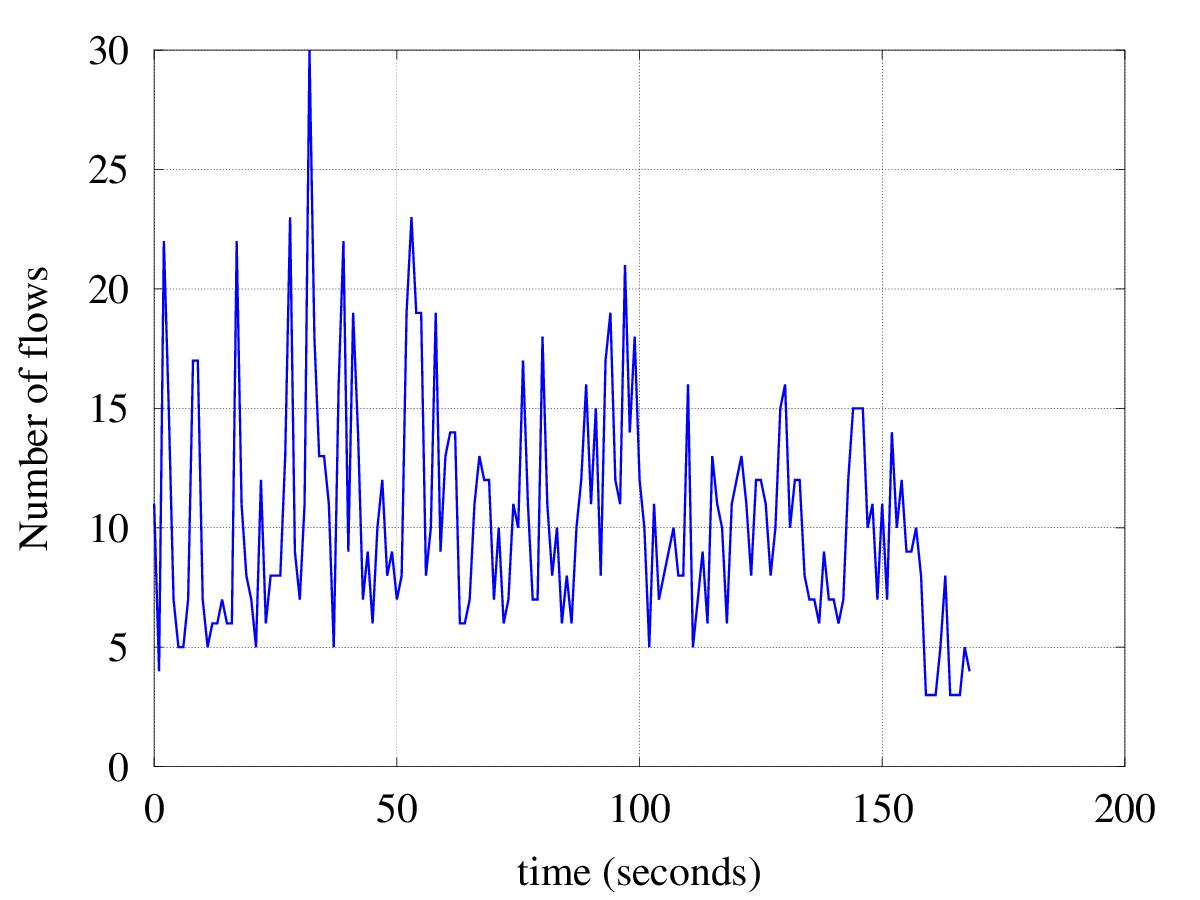
\includegraphics[height=55mm]{figures/Flow-qualification}}
%    \caption{Number of flows per second comparison between original and synthetic traces. Granularity of the plot: 1s}
%    \label{fig:mbps-comparison}
%\end{figure}

 

%\begin{figure}[H]
%        {\centering
%        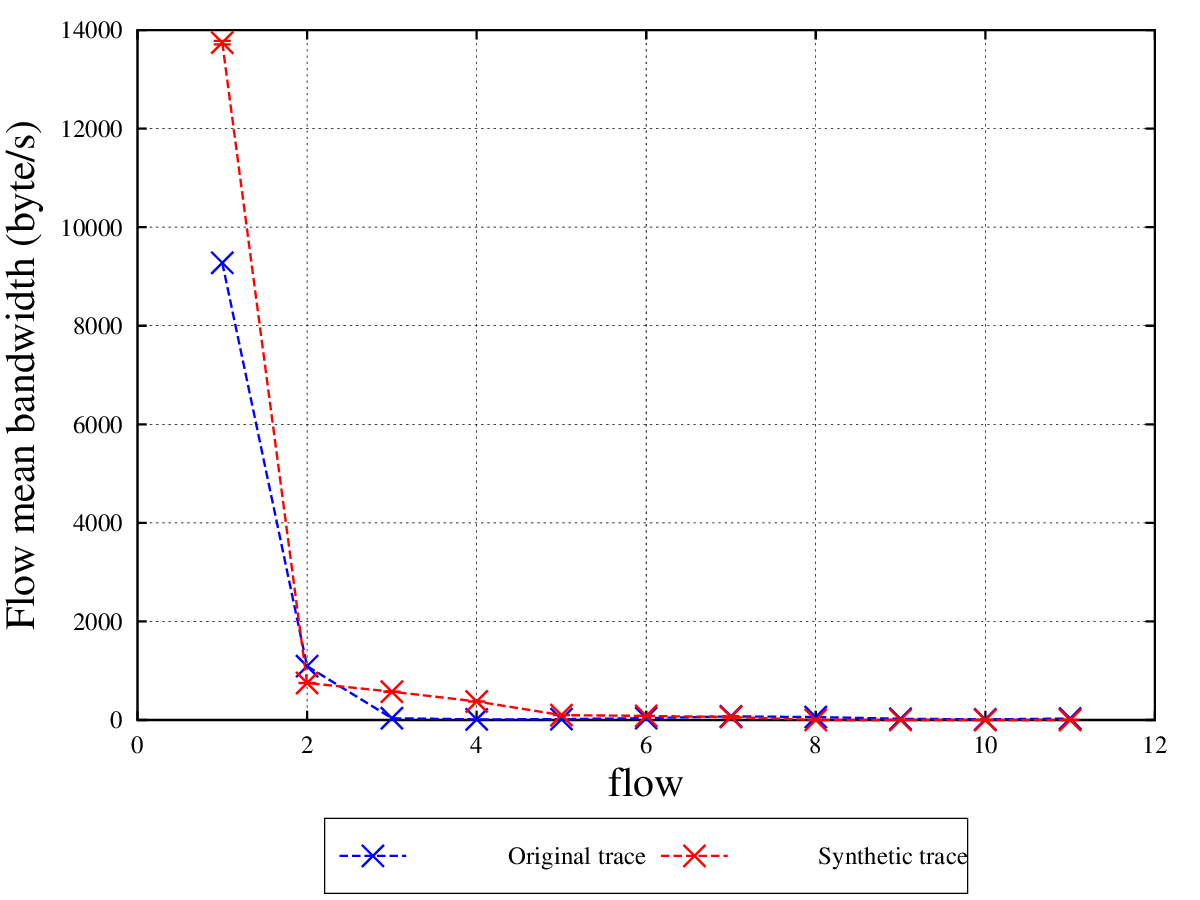
\includegraphics[height=55mm]{figures/qualification-bw.png}
%        \caption{}
%        \label{fig:sss}\par}
%\end{figure}

\begin{figure}[H]
        {\centering
        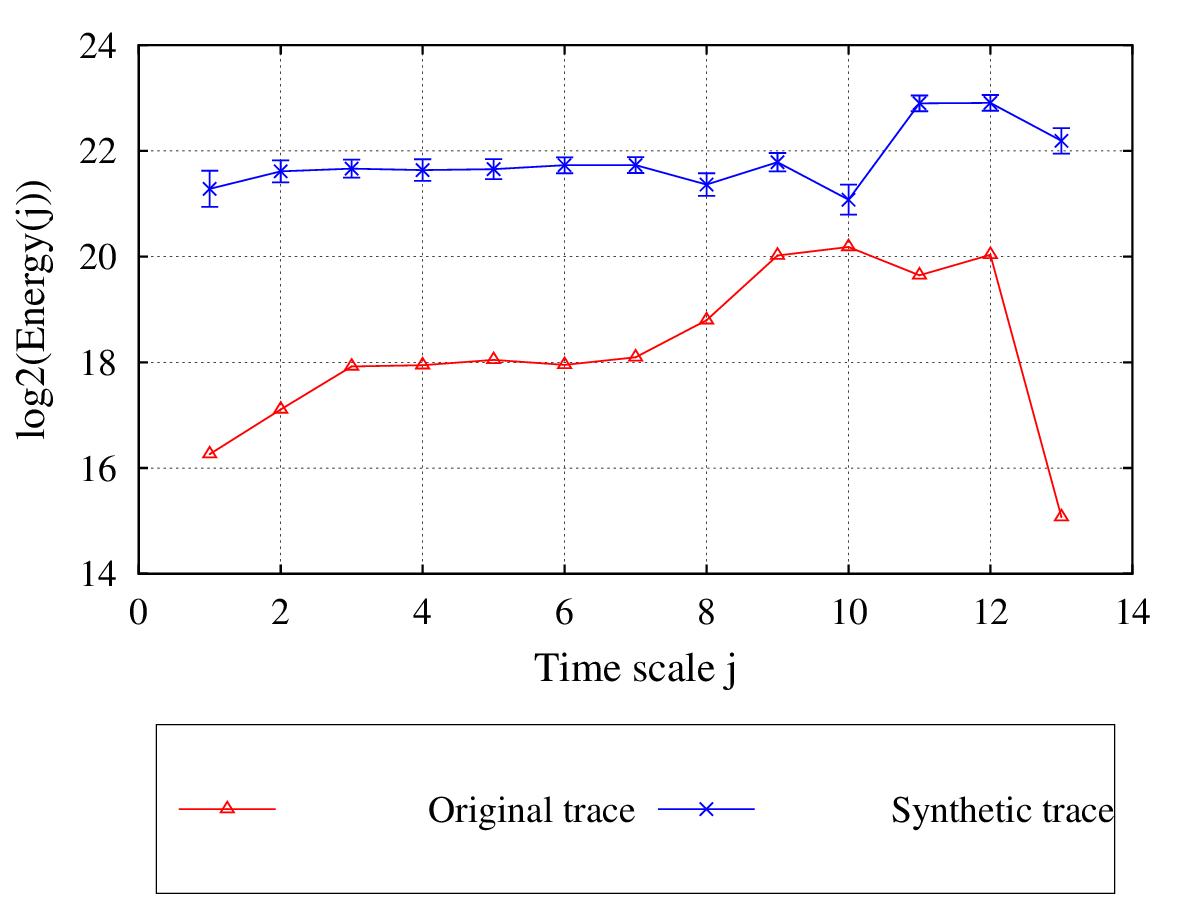
\includegraphics[height=50mm]{figures/qualification-WaveletMREA}
        \caption{Wavelet Multiresolution Energy Analysis of the original and synthetic traces}
        \label{fig:wavelet-mrea}\par}
\end{figure}


%%%%%%%%%%%%%%%%%%%%%%%%%%%%%%%%%%%%%%%%%%%%%%%%%%%%%%%%%%%%%%%%%%%%%%%%%%%%%
\section{Conclusion and future work}
\label{sec:conclusion-and-future-work}


The framework prototype was already able to generate a realistic (self-similar) Ethernet traffic. But, as expected, is still unable to represent well the particular features of the original traffic trace. This is a result of the, still, poor stochastic modelling. The next job will be implementing a significative modelling of the original traffic trace, through the specified methodology. We expect more significant results, them. Also, we will expand the framework to others workload platforms and compare the results. Packet acceleration could speed-up the performance, which may enable the reproduction of high-throughput traces. This can be implemented using DPDK. Finally, the results should be compared to Swing, on realism, similarity, and performance. This will give a measurement of how good is the framework, compared with others alternatives, and its strong and weak points. 

